% \documentclass{tufte-book}
\documentclass[a4paper,11pt]{book}
\usepackage{a4wide}
% \usepackage[utf8x]{inputenc}
\usepackage[unicode]{hyperref}
\usepackage[pdftex]{graphicx} % za slike
\usepackage{setspace}
\usepackage{textcomp}
\usepackage[version=3]{mhchem}
\usepackage{booktabs} % makes nice quality tables
\usepackage{emptypage}


% \usepackage{mathptmx}
\usepackage{palatino} 
\usepackage{pxfonts}
\usepackage{charter}
\usepackage{algorithmic} % for algorithms

\usepackage{amsopn}
\DeclareMathOperator*{\argmax}{\arg\,\max}

\renewcommand{\baselinestretch}{1.2}
\newcommand{\angl}[1]{(angl. {\em #1})}
\newcommand{\comment}[1]{#1}
\newcommand{\pd}[2]{\frac{\partial#1}{\partial#2}}
\newcommand{\plogp}[2]{{#1\over #2}\log_2{#1\over #2}}
\newcommand{\tr}{\intercal}
\newcommand{\mean}[1]{\overline{#1}}
\newcommand{\Var}{\mathrm{Var}}
\newcommand{\norm}[1]{\left\lVert#1\right\rVert}
\newcommand{\vect}[1]{\boldsymbol{#1}}

\newcommand{\chaptersummary}[1]{ {\em #1}}

\usepackage{color}
\definecolor{light-gray}{gray}{0.95}
% \newcommand{\text}{\rm}
\usepackage{listings}
\usepackage{url}
% \usepackage{program}

\newtheorem{teorem}{Teorem}

\usepackage[most]{tcolorbox}
\newcounter{testexample}
\usepackage{lipsum}

\def\R{\mathbb{R}}
\def\barwidth{3pt}
\def\exampletext{Example} % If English

\NewDocumentEnvironment{example}{ O{} }
{
\colorlet{colexam}{white!50!black} % Global example color
\newtcolorbox[use counter=testexample]{testexamplebox}{%
    % Example Frame Start
    empty,% Empty previously set parameters
    title={\exampletext: #1},% use \thetcbcounter to access the testexample counter text
    % Attaching a box requires an overlay
    attach boxed title to top left,
       % Ensures proper line breaking in longer titles
       minipage boxed title,
    % (boxed title style requires an overlay)
    boxed title style={empty,size=minimal,toprule=0pt,top=4pt,left=5mm,overlay={}},
    coltitle=colexam,fonttitle=\bfseries,
    before=\par\medskip\noindent,parbox=false,boxsep=0pt,left=5mm,right=0mm,top=2pt,breakable,pad at break=0mm,
       before upper=\csname @totalleftmargin\endcsname0pt, % Use instead of parbox=true. This ensures parskip is inherited by box.
    % Handles box when it exists on one page only
    overlay unbroken={\draw[colexam,line width=\barwidth] ([xshift=2pt]title.north west) -- ([xshift=2pt]frame.south west); },
    % Handles multipage box: first page
    overlay first={\draw[colexam,line width=\barwidth] ([xshift=-0pt]title.north west) -- ([xshift=-0pt]frame.south west); },
    % Handles multipage box: middle page
    overlay middle={\draw[colexam,line width=\barwidth] ([xshift=-0pt]frame.north west) -- ([xshift=-0pt]frame.south west); },
    % Handles multipage box: last page
    overlay last={\draw[colexam,line width=\barwidth] ([xshift=-0pt]frame.north west) -- ([xshift=-0pt]frame.south west); },%
    }
\begin{testexamplebox}}
{\end{testexamplebox}\endlist}


\NewDocumentEnvironment{summary}{ O{} }
{
\colorlet{colexam}{red!55!black} % Global example color
\newtcolorbox{summarybox}{%
    % Example Frame Start
    empty,% Empty previously set parameters
    % Attaching a box requires an overlay
    coltitle=colexam,fontupper=\bfseries,
    before=\par\medskip\noindent,parbox=false,boxsep=0pt,left=5mm,right=0mm,top=2pt,breakable,pad at break=0mm,
       before upper=\csname @totalleftmargin\endcsname0pt, % Use instead of parbox=true. This ensures parskip is inherited by box.
    % Handles box when it exists on one page only
    overlay unbroken={\draw[colexam,line width=\barwidth] ([xshift=2pt]frame.north west) -- ([xshift=2pt]frame.south west); },
    % Handles multipage box: first page
    overlay first={\draw[colexam,line width=\barwidth] ([xshift=-0pt]frame.north west) -- ([xshift=-0pt]frame.south west); },
    % Handles multipage box: middle page
    overlay middle={\draw[colexam,line width=\barwidth] ([xshift=-0pt]frame.north west) -- ([xshift=-0pt]frame.south west); },
    % Handles multipage box: last page
    overlay last={\draw[colexam,line width=\barwidth] ([xshift=-0pt]frame.north west) -- ([xshift=-0pt]frame.south west); },%
    }
\begin{summarybox}}
{\end{summarybox}\endlist}

\NewDocumentEnvironment{guide}{ O{} }
{
\colorlet{colexam}{yellow!55!black} % Global example color
\newtcolorbox{guidebox}{%
    % Example Frame Start
    empty,% Empty previously set parameters
    % Attaching a box requires an overlay
    coltitle=colexam,fontupper=\footnotesize,
    before=\par\medskip\noindent,parbox=false,boxsep=0pt,left=5mm,right=0mm,top=2pt,breakable,pad at break=0mm,
       before upper=\csname @totalleftmargin\endcsname0pt, % Use instead of parbox=true. This ensures parskip is inherited by box.
    % Handles box when it exists on one page only
    overlay unbroken={\draw[colexam,line width=\barwidth] ([xshift=2pt]frame.north west) -- ([xshift=2pt]frame.south west); },
    % Handles multipage box: first page
    overlay first={\draw[colexam,line width=\barwidth] ([xshift=-0pt]frame.north west) -- ([xshift=-0pt]frame.south west); },
    % Handles multipage box: middle page
    overlay middle={\draw[colexam,line width=\barwidth] ([xshift=-0pt]frame.north west) -- ([xshift=-0pt]frame.south west); },
    % Handles multipage box: last page
    overlay last={\draw[colexam,line width=\barwidth] ([xshift=-0pt]frame.north west) -- ([xshift=-0pt]frame.south west); },%
    }
\begin{guidebox}}
{\end{guidebox}\endlist}

\newcommand{\ifguide}[1]{\begin{guide}#1\end{guide}}
\renewcommand{\ifguide}[1]{}


\lstnewenvironment{python}[1][]{
\lstset{
language=python,
basicstyle=\ttfamily\footnotesize\setstretch{1},
stringstyle=\color{red},
showstringspaces=false,
alsoletter={1234567890},
otherkeywords={\ , \}, \{},
keywordstyle=\color{blue},
emph={access,and,break,class,continue,def,del,elif,else,%
except,exec,finally,for,from,global,if,import,in,is,%
lambda,not,or,pass,print,raise,return,try,while},
emphstyle=\color{black}\bfseries,
emph={[2]True, False, None, self},
emphstyle=[2]\color{green},
emph={[3]from, import, as},
emphstyle=[3]\color{blue},
upquote=true,
morecomment=[s]{"""}{"""},
commentstyle=\color{red}\slshape,
emph={[4]1, 2, 3, 4, 5, 6, 7, 8, 9, 0},
emphstyle=[4]\color{blue},
literate=*{:}{{\textcolor{blue}:}}{1}%
{=}{{\textcolor{blue}=}}{1}%
{-}{{\textcolor{blue}-}}{1}%
{+}{{\textcolor{blue}+}}{1}%
{*}{{\textcolor{blue}*}}{1}%
{!}{{\textcolor{blue}!}}{1}%
{(}{{\textcolor{blue}(}}{1}%
{)}{{\textcolor{blue})}}{1}%
{[}{{\textcolor{blue}[}}{1}%
{]}{{\textcolor{blue}]}}{1}%
{<}{{\textcolor{blue}<}}{1}%
{>}{{\textcolor{blue}>}}{1},%
% framexleftmargin=1mm, framextopmargin=1mm, frame=shadowbox, rulesepcolor=\color{blue},#1
}}{}

\lstset{ %
language=Python,
basicstyle=\ttfamily\setstretch{1},
backgroundcolor=\color{light-gray}
}

% include hyperlinks
\usepackage{hyperref}

\usepackage[backend=biber]{biblatex}
\addbibresource{notes.bib}


\title{Machine Learning for Data Science 1 \\
\small (lecture notes, only for internal use)}
\author{Blaž Zupan, Erik Štrumbelj}
\date{\today}


\begin{document}

\maketitle
\tableofcontents

\begin{refsection}
\chapter{Introduction}

\begin{summary}
Machine learning is a set of approaches that can detect patterns in the data. Types of machine learning include predictive and descriptive reinforcement learning. Two major classes of predictive learning are classification and regression. Examples of unsupervised learning approaches include principal component analysis, clustering, and dimensionality reduction. We can formalize predictive and descriptive learning as density estimation, where we develop probabilistic formulations of the form $p(y|\vect{x}_i,\mathcal{D})$ for predictive, and formulations of the form $p(y|\mathcal{D})$ for unsupervised learning. Resulting probabilistic models $p(y|\vect{\theta})$ or $p(y|\vect{x}_i; \vect{\theta})$ may include fixed number of parameters, or their number may vary according to the size of the training data. Interesting concepts in machine learning include the curse of dimensionality, inductive bias, overfitting, model selection, and absence of a universally best model that would fit all kinds of problem domains.~\footnote{These lecture notes follow Chapter 1 from~\citet{2012-Murphy}. Recommended additional reading is Chapter 2 from~\citet{ESL}.}
\end{summary}

\ifguide{
The purpose of this chapter is to introduce students to the basic definitions, general types of machine learning problems, things to consider in practical applications and fundamental concepts (curse of dimensionality, no-free-lunch theorem). We can also introduce kNN. Together with linear and logistic regression and PCA, which they already know, we have enough variety to cover the illustrative examples we need for this chapter.

Keep in mind that the Intro to DS course will already provide students with a practitioner's (black-box) understanding of the application of predictive models (classification/regression), clustering and dimensionality reduction, and dealing with missing values. This includes a black-box understanding of train/test and $k$-fold CV estimation of generalization error. Principles of Uncertainty will also give them a fundamental understanding of bootstrap non-parametric inference, maximum likelihood inference, Bayesian inference, and classical hypothesis testing. And a fundamental understanding of the following models: linear regression, logistic regression, PCA.
}

\section{The Purpose of Machine Learning}

\ifguide{
The students will already be used to the statistical notation of data, models (likelihoods), etc. ($y$, $x$, $p(y|x)$, etc.). It is important that the ML course continues with this to strengthen the student's abstraction. With a good understanding of $p(x,y)$ and $p(y|x)$ it becomes much easier to characterize terms that are commonly used in practice, such as classification, (un)supervised learning, regression, etc. (as we do below).
}

Machine learning is about learning models from data. More abstractly, given the training data $\mathcal{D}$, we would like to use the data to infer probability distributions. In other words, we would like to build models of the process $p(y)$ that generated the data.

The general task of learning $p(y|\mathcal{D})$, that is, inferring the conditional distribution of variables that define the processes given the data is very complex. In practice, we are, in most cases, not even interested in this general task. Instead, we are interested only in certain aspects of the distribution, and for these, apply specific types of machine learning, like classification, regression, or clustering.

In terms of applications, machine learning is a branch of artificial intelligence that provides algorithms that can automatically learn from experience without being explicitly programmed. While we will focus on theoretical aspects of machine learning, the reader of this text should place these in practical contexts and consider the tasks such as data acquistion, data cleaning, feature engineering, data cleaning and preprocessing, data visualisation, scoring and estimating the quality and utility of the developed models, and finally, their inclusion within working software and decision support systems. While practically of utmost importance, these engineering aspects will not be at the focus of this course.

\section{Types of Machine Learning}

\subsection*{Supervised learning}

Often, we are only interested in how a subset of variables is generated, while the remaining variables are used to explain the behavior of the variables of interest: $\{y_i, \vect{x}_i\}_{i=1}^n$. This is {\em supervised learning}, also known as {\em predictive learning} or {\rm predictions}. Here, $y$ is referred to as {\em response variable}, and $\vect{x}$ represents a vector of {\em features}. Depending on a branch of science that deals with machine learning, the dependent variable may also be referred to as a target variable, dependent variable (statistics), or label or class variable (machine learning). The independent variables are often referred to as covariates, independent variables, and predictors (statistics), or features and attributes (machine learning). Supervised learning starts with the training data, which includes $n$ pairs of instantiations of independent and dependent variables. The goal is to learn about $p(y|\vect{x})$ so that we can make predictions for future or unobserved values of independent variable $y$ for any combination of dependent variables $\vect{x}$ (see Table~\ref{tab:iris-sample}).

When $y$ is a nominal variable, we refer to this type of supervised learning as {\em classification}. When the nominal variable is two-valued, we deal with {\em binary classification}, and when the domain of the nominal variable includes three or more values, we refer to the problem as {\em multiclass classification}. When $y$ is continuous, we refer to the problem as {\em regression}. Less common cases consider a count or ordinal dependent variable, where we refer to the suitable approaches as {\em count regression} and {\em ordinal regression}, respectively. In most cases, the dependent variable $y$ will be a scalar, and we will refer to such cases as {\em univariate} classification or regression. When $y$ is a vector, we will refer to the problem as {\em multivariate} classification or regression.

Note that while various machine learning approaches specialize in a particular case, it is often easy to generalize a specific approach to deal with other types of the dependent variable. For instance, it is not difficult to adapt classification trees to the regression problems, or even to extend this approach to address multivariate learning.

\begin{table}
\caption{A small sample from the famous Iris data set, where Iris flowers are described with four numerical features and are labeled with Iris species. A possible task for this data set is supervised learning, with aim to build a model that predicts species from leaf morphology.}
\label{tab:iris-sample}
\begin{center}
\begin{tabular}{ccccl}
\toprule
sepal length & sepal width & petal length & petal width & iris \\
\midrule
4.4 & 2.9 & 1.4 & 0.2 & Iris-setosa \\
4.8 & 3.4 & 1.6 & 0.2 & Iris-setosa \\
5.4 & 3.9 & 1.3 & 0.4 & Iris-setosa \\
5.2 & 2.7 & 3.9 & 1.4 & Iris-versicolor \\
6.0 & 2.2 & 4.0 & 1.0 & Iris-versicolor \\
\bottomrule
\end{tabular}
\end{center}
\end{table}

\subsection*{Unsupervised learning}

We are using {\em unsupervised learning} when our problem does not include any response variable, that is, when the observations are not labelled. The goal of such learning is again to understand the data generative process $p(y)$, or at least to understand part of its structure.

A common approach to understanding the distribution $p(y)$ is to explain it with a smaller number of factors $\theta$, that is, to learn $p(y|\theta)$, effectively projecting the data into a lower-dimensional space. We refer to such procedure as {\em dimensionality reduction}. An extreme example of dimensionality reduction is {\em clustering}, when we try to explain $p(y)$ with a single nominal factor (see Fig.~\ref{fig:tsne-sc}). In essence, we are trying to group, or cluster, observations.

\begin{figure}[htbp]
\centering{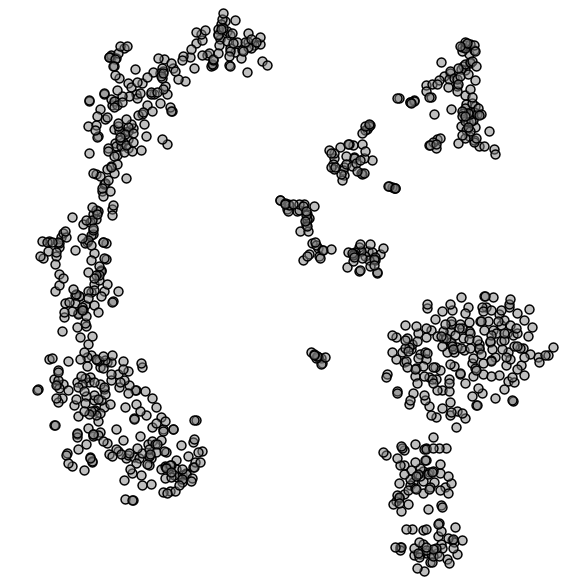
\includegraphics[width=8cm]{figures/intro-tsne-single-cell.png}}
\caption{A two-dimensional visualisation of blood cells, originally described with expressions of thousands of features. The visualisation was constructed using t-SNE dimensionality reduction, and exposes potential clusters that need to be further analyzed.}
\label{fig:tsne-sc}
\end{figure}

\subsection*{Reinforcement learning}

Reinforcement learning is about learning actions of software agents in an environment where the goal is to maximize reward. An example of reinforcement learning is to learn the actions of a robot that travels through the maze and receives sensor input. A reward, in this case, could be time spent in a maze. Reinforcement learning is different from supervised learning in not requiring labeled input. Instead, reinforcement learning aims to find the balance between the exploration of uncharted territory and the exploitation of current knowledge. While we will focus on unsupervised and supervised learning in this course, we will only dive into reinforcement learning in one of our final sessions.


\section{Models and Learning}

A {\em model} $\mathcal{H}$ is in the most abstract sense a collection of distributions (densities, functions, ...). The elements of a model depend on our task.

\begin{example}[Simple linear regression - statistical model]
The simple linear regression is a set of densities \\
$\mathcal{H} =\left\lbrace p(y|\vect{x},\vect{\b},\alpha, \sigma)  = dnorm(\vect{\b}\vect{x} + \alpha, \sigma^2), \vect{\b}, \alpha \in \R, \sigma > 0 \right\rbrace$
\end{example}

\begin{example}[Simple linear regression - function approximation]
The simple linear regression is a set of functions
$\mathcal{H} =\left\lbrace f(\vect{x},\vect{\b},\alpha) = \vect{\b} \vect{x} + \alpha, \vect{\b}, \alpha \in \R \right\rbrace$
\end{example}

It is important to reinforce the view of a model as a set of hypotheses. Learning is the process of expressing a preference for certain hypotheses based on evidence (data). Choosing a particular machine learning algorithm, or in other words, choosing a particular model means expressing a preference for a certain type of hypothesis. The logistic regression model, in its basic form, will construct a model which will linearly separate the parameter space of the data instances to, prefarably, separate the data instances from either of the two classes. Separation plane constructed by classification trees may be much more complex and, implicitly, require many more parameters for its descriptions. The choice of the model also entails the choice of the complexity of the hypothesis, which in turn is related to the goodness of fit, overfitting, explainability, and other issues we expose in the text below.

A model is often also referred to as a hypothesis or set of hypotheses. Learning is often referred to as training the model, fitting the model/parameters, estimation.

{\em Learning} is the process of selecting elements of $\mathcal{H}$ based on some utility and using data. This is general. In practice, we can select a single element (a single density, function, distribution; as in the two function approximation examples above), a set of elements or even weight each element, for example, a distribution across all elements, as in Bayesian approaches.

Learning is in most cases just a problem in {\em computation} to be addressed through mathematical, numerical, algorithmic procedures. For parametric models, we typically do {\em least-squares} or {\em maximum likelihood} estimations to obtain {\em point estimates} of the parameters of the model. That is, by learning, we select a single model. Learning thus becomes an {\em optimization} problem, or {\em Bayesian inference}, which is an {\em integration} or optimization problem, if we do some sort of {\em structural approximation} or {\em MAP}. \


\subsection*{Parametric and Nonparametric Models}

If the set $\mathcal{H}$ can be parametrized with a finite number of parameters, we call the model {\em parametric}. Otherwise, it is {\em nonparametric}. A parametric model captures all information about the properties of the data within its fixed number of parameters. Predictions using non-parametric models require knowledge about the current state of the system, that is, require access to the current data.

\begin{example}[1-nearest neighbor model - a nonparametric model]
$\mathcal{H} = \lbrace$ all functions $f$ that can be expressed with a set of points (data instances) and the rule that $f(\vect{x}) = y_i$ of point $x$ nearest to $x_i$, according to a chosen distance metric$\rbrace$ (see Fig.~\ref{fig:1-nn})
\end{example}

\begin{figure}[htbp]
\centering{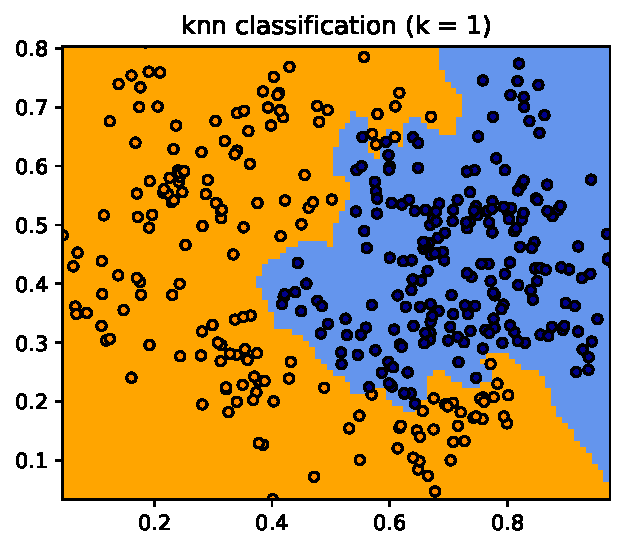
\includegraphics[width=0.6\linewidth]{figures/intro-knn-1.pdf}}
\caption{Decision boundary of a 1-nearest neighbor model trained on a two-featured binary classification data set with 380 data instances (170 in one class and 210 in the other) as shown on a figure. The decision boundary is complex and may substantially change with any addition on removal of the data.}
\label{fig:1-nn}
\end{figure}

Parametric models are easier to compute than non-parametric models. Non-parametric models are often more complex and grow with data. Parametric models depend on the data only through a finite number of parameters, while in non-parametric models, the complexity of the model depends on the training set. Researchers mostly prefer parametric models because it may be easier to estimate its parameters, easier to perform predictions, and easier to tell a story about the data according to a parametric model (e.g., sensitivity analysis, effects of the changes in parameters, parameter interactions). In this sense, parametric models are more prone to interpretation by domain experts. In parametric models, the parameter estimates may have better statistical properties compared to those of non-parametric regression.

Parametric models make stronger assumptions about the data; the learning may be successfull if these assumptions are valid, but the inferred predictors may fail if these assumptions are violated. Think of modeling a sine curve with a linear regression model. A non-parametric algorithm is computationally slower but makes fewer assumptions about the data. In (overly) simplified view, the trade-offs between parametric and non-parametric algorithms are in computational cost and accuracy.

Notice that non-parametric models are related to {\em lazy learning}. Lazy learning methods generalize the training data at the time of prediction. This type of learning is an alternative to {\em eager learning}, where the system tries to generalize the training data before receiving queries. An example of the lazy learner is a $K$-nearest neighbor algorithm. Lazy learners may have an advantage in real-time environments, where the training data changes in time and models trained in the past become obsolete in a relatively short time due to emergent new data and changes of the distributions and underlying processes that generated the data.

\ifguide{
It is good for the instructor to be aware that this definition of parametric models is operational but not rigorous. In fact, it is flawed. The set of all possible probability measures has the same cardinality as R. In other words, even a nonparametric model can be written as a model with a single real parameter. Assuming smoothnes solves the technical difficulties, but all of this is outside the scope of this course.
}

\section{Challenges of Applied Machine Learning}

\subsection*{Model Evaluation and Selection}

In theory, assuming uniform distribution over all possible datasets, there is no single best model. In fact, and again, in theory, no model is strictly better than any other model. This is in the literature referred to as {\em no free lunch theorem}, which states that any two optimization algorithms are equivalent when their performance is averaged across all possible problems~\citep{2005-Wolpert-Macready}. 

In practice, however, some characteristics are more common in datasets, so some models and algorithms perform better on average because their assumptions ({\em inductive bias}) better match the characteristics of the data generating process.

The above makes {\em model selection} a key part of applied machine learning. In order to train a model, we should define some measure of utility we would like to optimize. A trivial approach is then to select the model with the best utility on our available data. However, estimating the model's utility on the data it was trained on is biased and optimistic. In practice, the model's utility on the training data (so-called {\em in-sample} error) may be substantially better than on independent test data ({\em out-of-sample} error or {\em generalization error}). This effect is also known as {\em overfitting}, and it is something that we want to both detect and prevent.

\begin{figure}
\centering{
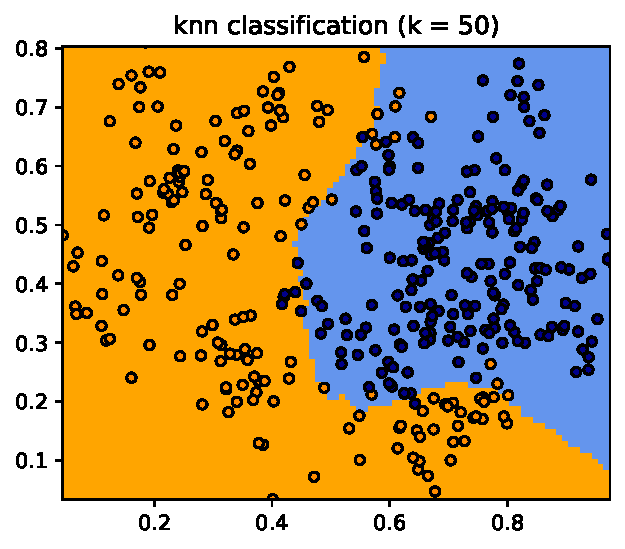
\includegraphics[width=0.47\linewidth]{figures/intro-knn-50.pdf}
\hfill
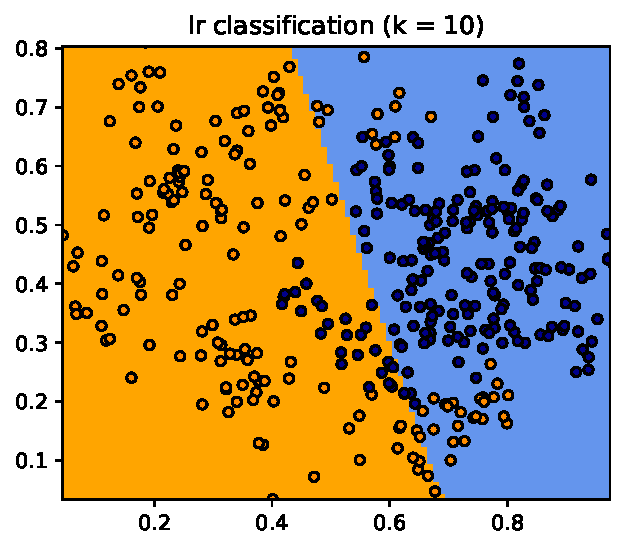
\includegraphics[width=0.47\linewidth]{figures/intro-logreg.pdf}
}
\caption{Decision boundary on a two-featured binary classification data set as inferred by nearest neighbor algorithm with K=50 and by logistic regression. Which model would perform better on new data?}
\label{fig:1-nn}
\end{figure}

\subsection*{Overfitting}

Overfitting occurs when machine learning model trained on a (limited) data set captures noise of the data instead of the underlying data generation processes. This modelling error occurs when an inferred hypothesis is too closely fit to a limited set of data points, or when a model is too complex for a given data (e.g., Fig.~\ref{fig:tree-overfit}). 

\begin{figure}[htbp]
\centering{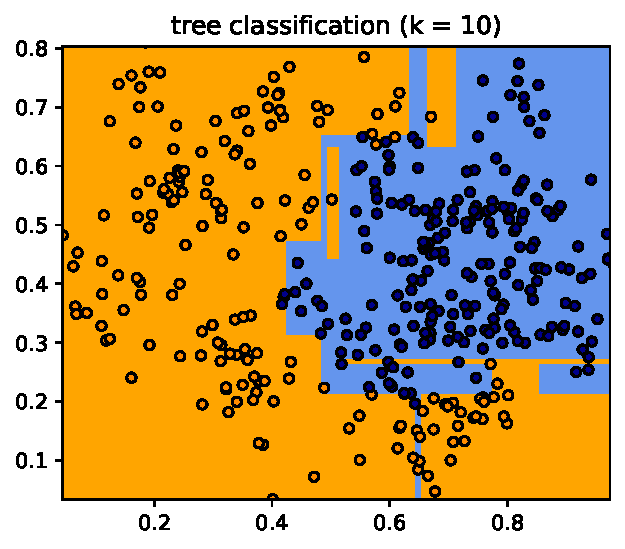
\includegraphics[width=0.6\linewidth]{figures/intro-tree-10.pdf}}
\caption{Classification trees would often overfit the training data. Figure shows decision boundary of a tree where the allowed maximum tree depth was 10. The decision boundary is complex and often covers single-case exceptions.}
\label{fig:tree-overfit}
\end{figure}

\begin{figure}[htbp]
\centering{
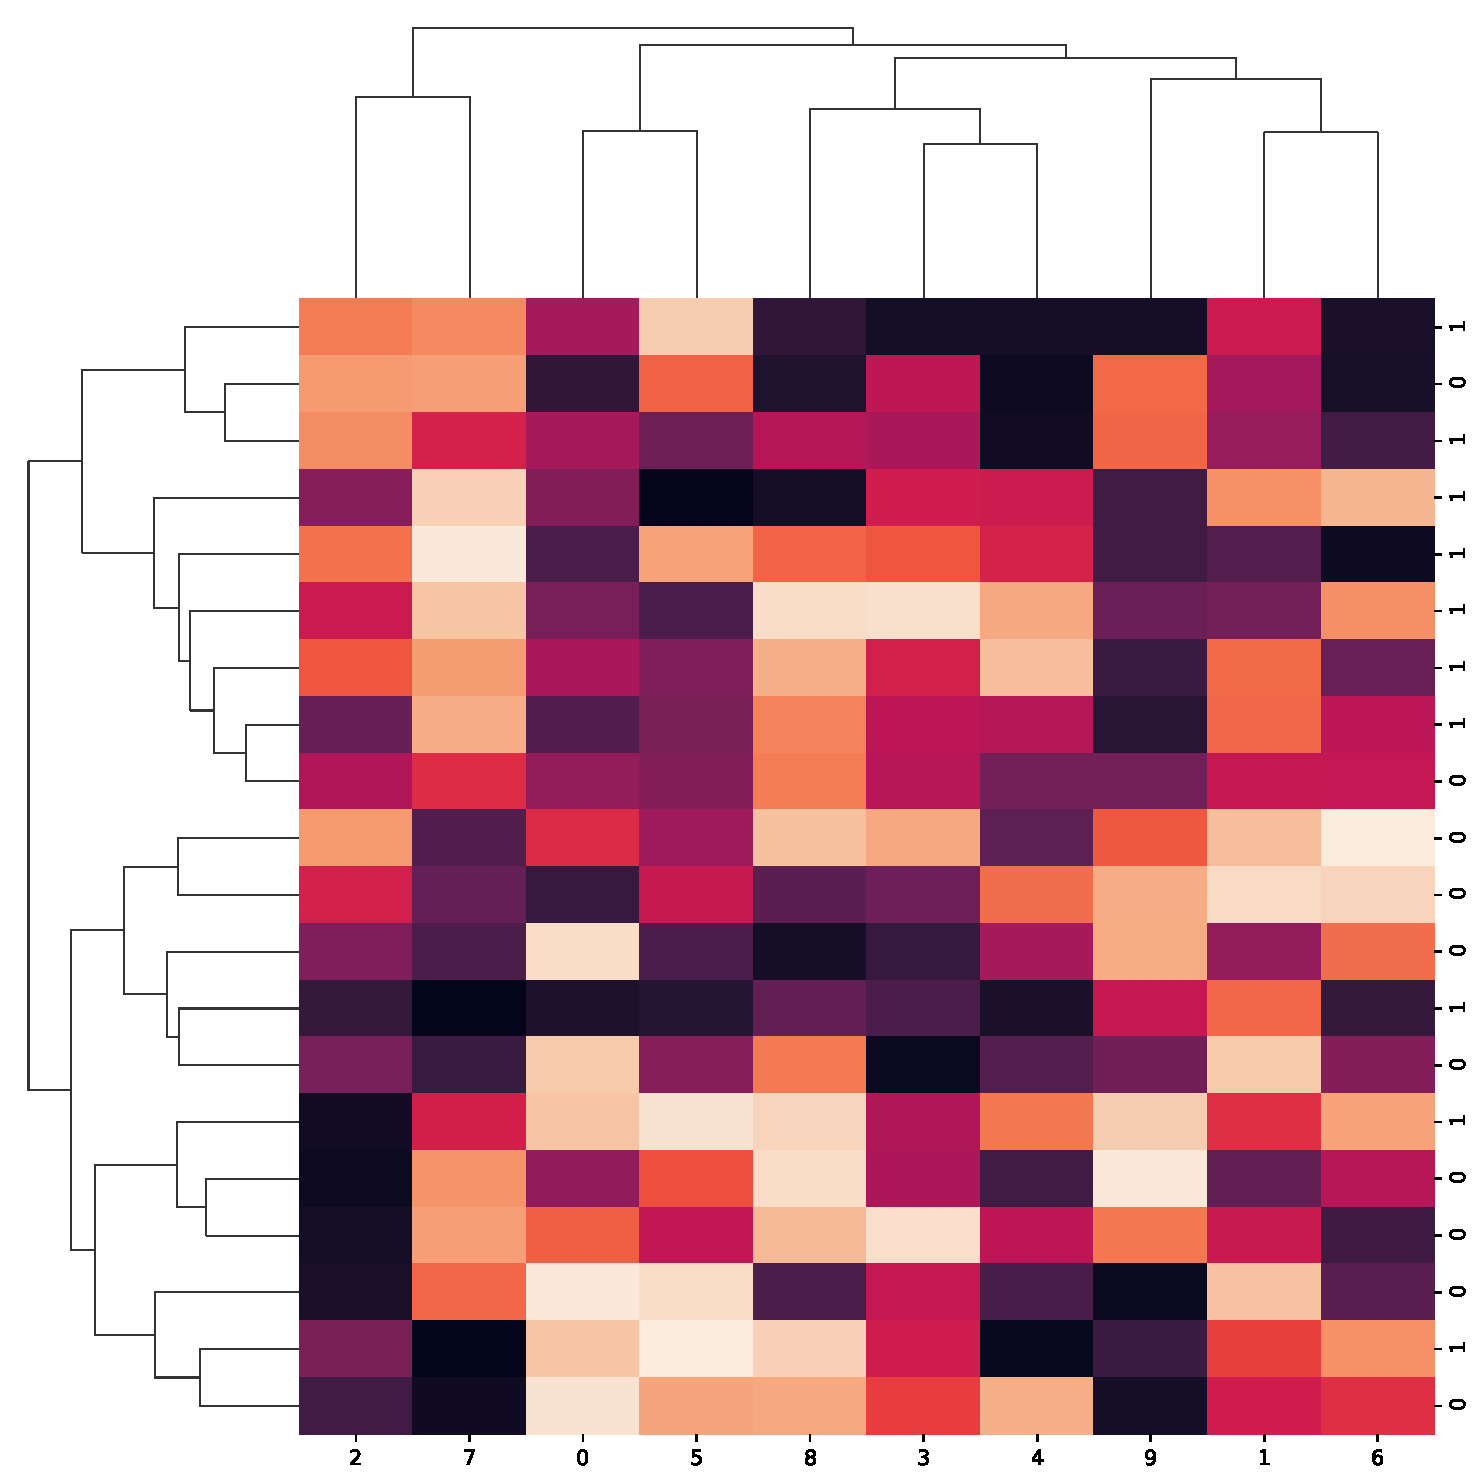
\includegraphics[width=0.47\linewidth]{figures/intro-heatmap-default.pdf}
\hfill
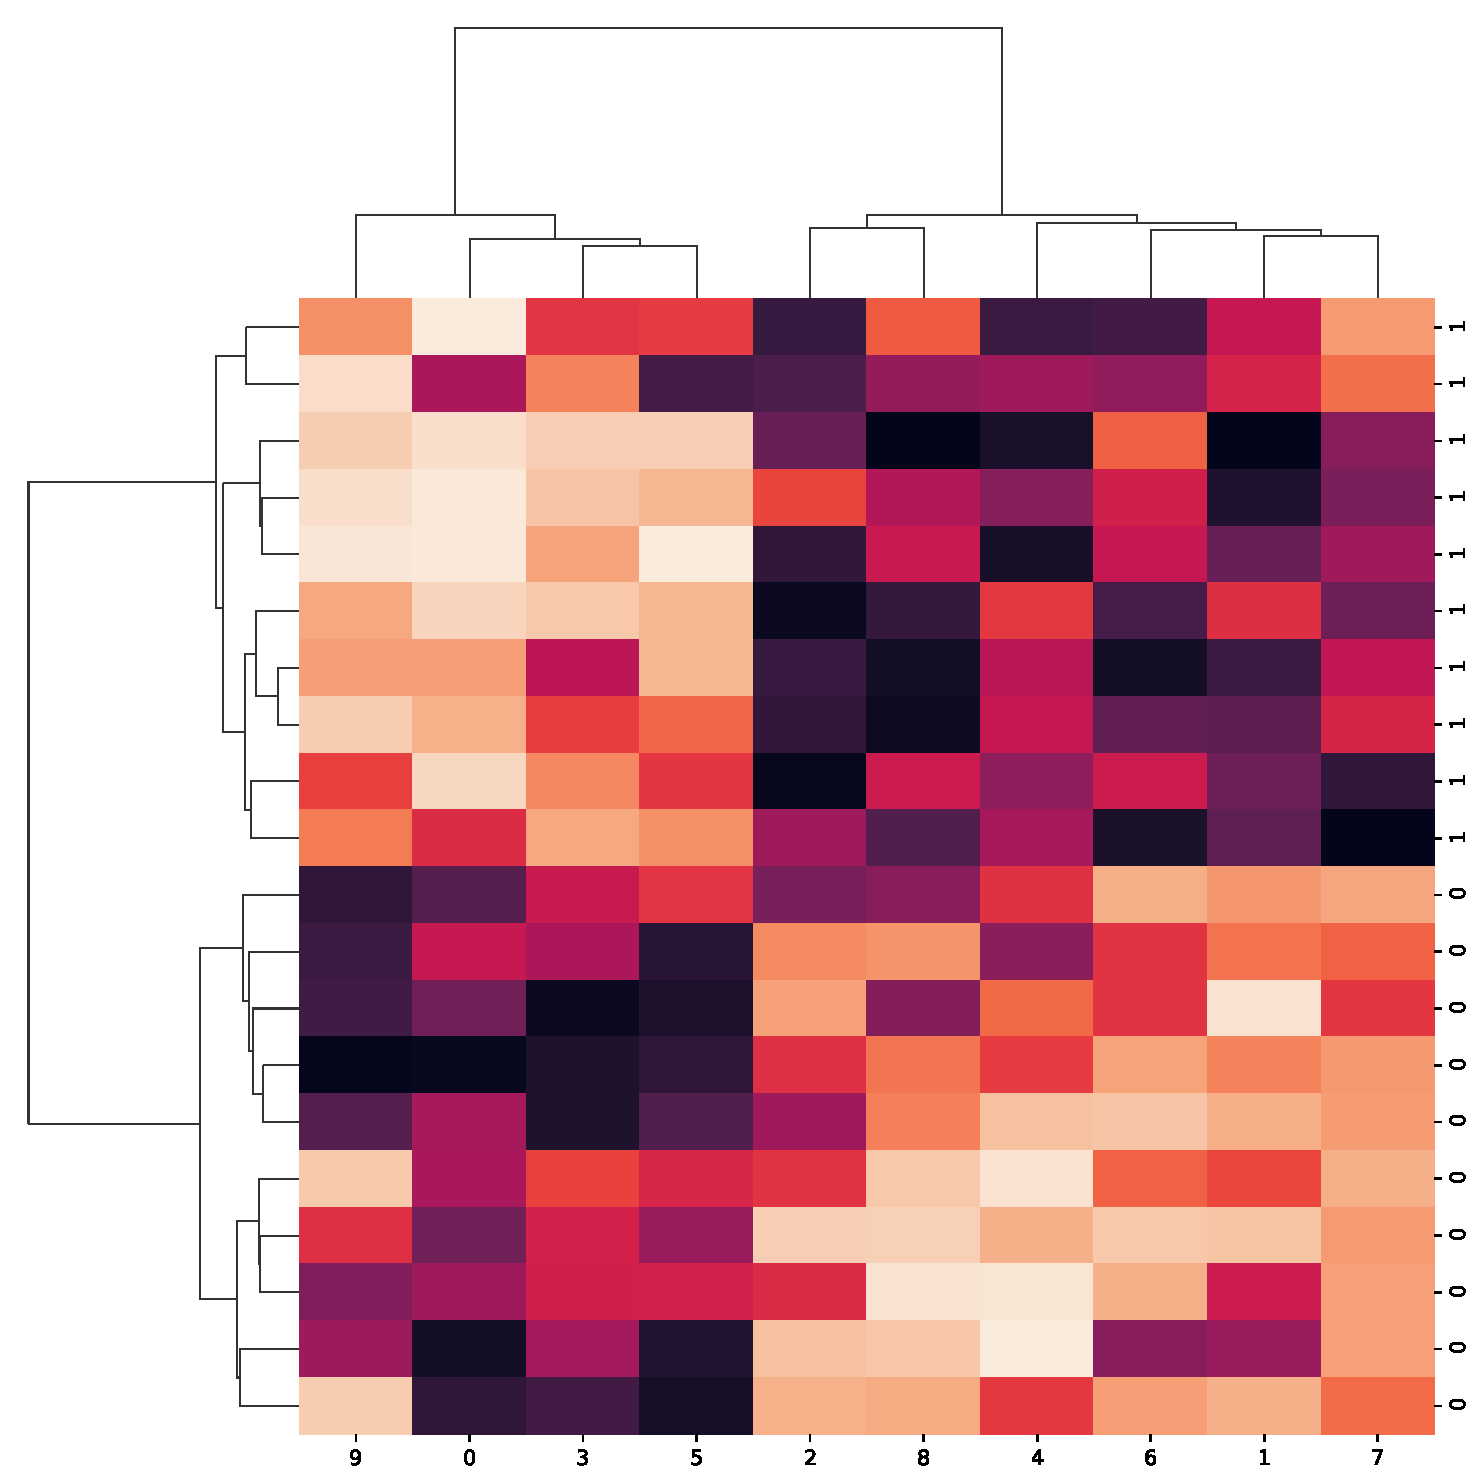
\includegraphics[width=0.47\linewidth]{figures/intro-heatmap-fss.pdf}
}
\caption{Co-clustering of a random data set with 20 instances and 10 features (left), and co-clustering of a similar data set with 10000 features, of which 10 features were selected that best correlate with a binary label (right). Notice a clear pattern of colors and shades in the right heatmap, which should not be there if correct data preprocessing procedures were applied.}
\label{fig:heatmaps-overfitting}
\end{figure}

The related practical challenges include knowing when overfitting occurs and finding the right remedy for overfitting. Another challenge is to avoid modeling procedures that led to overfitting. None of these challenges is trivial, and beginners or even quite experienced practitioners often make mistakes that lead to overfitting and consequentially report over-optimistic scores for their modeling procedures. For instance, it has been found that some (if not most) of significant reports on the analysis of microarray gene expression data sets at the break of the century included overfitting~\citep{2003-Simon}. Common reported mistakes included feature selection before cross-validation or class label-informed feature selection before data visualization. Reports on good accuracies are, despite teachings in data science, present also in recent literature, as reported by Vandewiele et al.~\citep{2019-Vandewiele}. The authors examined reports on the analysis of a collection of electrohysterogram signals. There, related reports oversampled the data prior to cross-validation, and hence falsely obtained almost perfect accuracies.


\subsection*{Model Complexity and Effective Number of Parameters}

More complex models are more likely to overfit (see Figs.~\ref{fig:tree-depth-overfit} and \ref{fig:knn-learning-curve}), but the ``right'' complexity of the model may depend on the amount of data we have (see Fig.~\ref{fig:lr-overfitting}). In parametric models, especially linear models, the model's complexity easily be measured in terms of the number of parameters (or degrees of freedom). For nonparametric models the theory is more complex ({\em e.g.}, Vapnik–Chervonenkis dimension) and introduces the concept of the {\em effective number of parameters}. Typically, nonparametric models have a higher number of effective parameters and are thus able to better fit the data but also more prone to overfitting. But they are more difficult to interpret.

\begin{figure}[htbp]
\centering{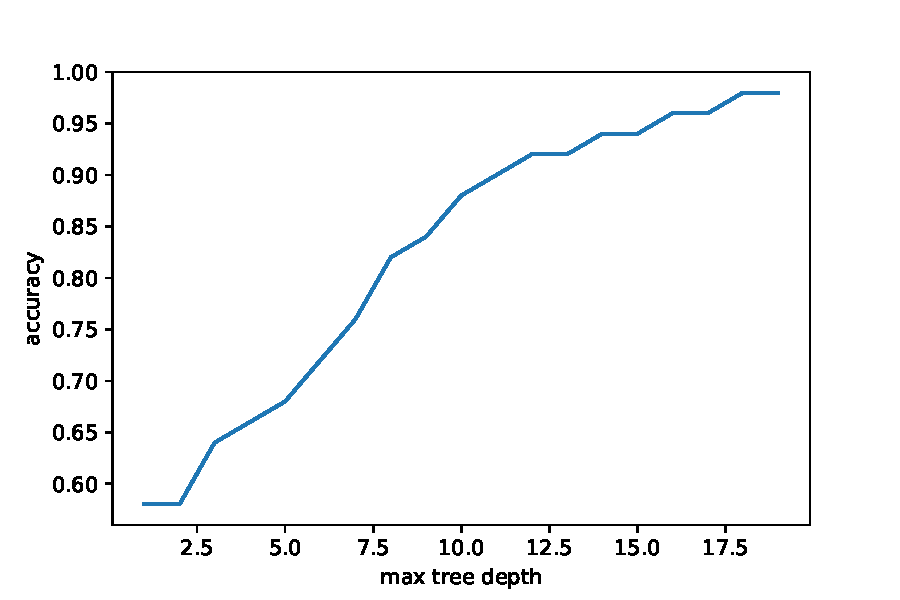
\includegraphics[width=0.6\linewidth]{figures/intro-tree-overfit-depth.pdf}}
\caption{A classification tree accuracy on a random class-balanced binary classification data set with one feature and 50 data instances. Trees were grown to a specified maximal depth. More complex trees better fit the training data.}
\label{fig:tree-depth-overfit}
\end{figure}

\begin{figure}[htbp]
\centering{
\centering{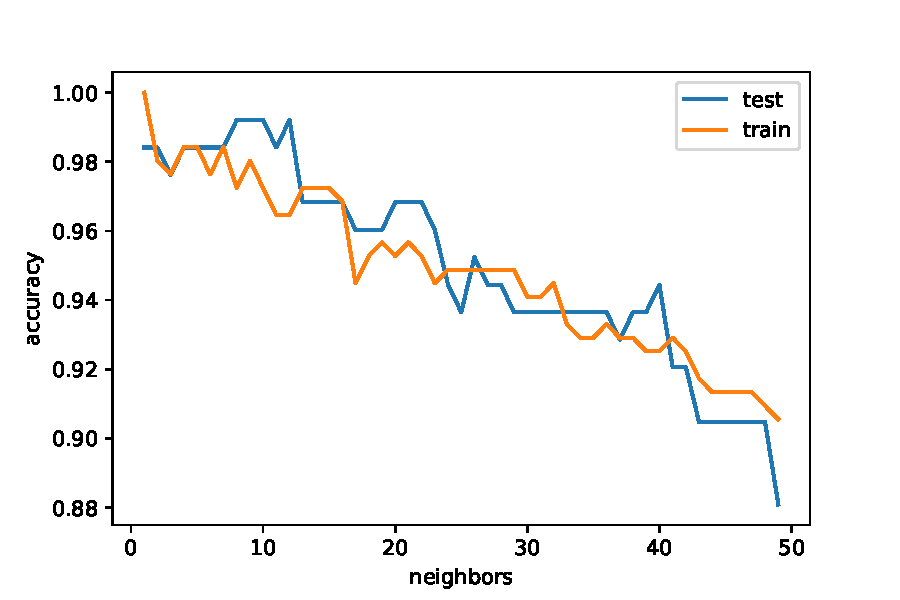
\includegraphics[width=0.6\linewidth]{figures/intro-knn-learning-curve.pdf}}
}
\caption{A training and test-set tradeoff for $k$-nearest neighbor model. On the training data, the accuracy falls with raising $k$, while on the test data set the accuracy peaks at around $k=10$. Hyper-parameter estimation is one of the key issues when selecting the most appropriate model.}
\label{fig:knn-learning-curve}
\end{figure}


\begin{figure}[htbp]
\centering{
\centering{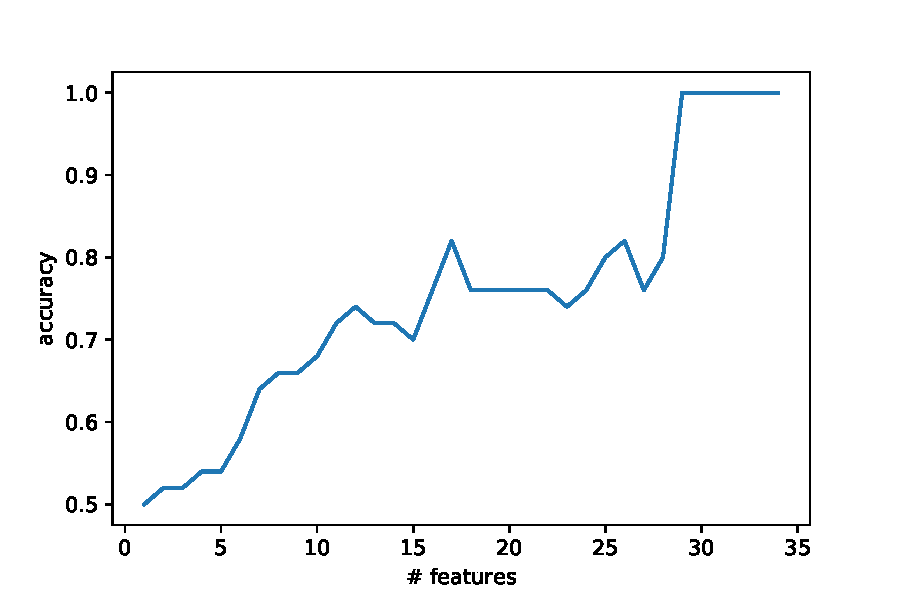
\includegraphics[width=0.6\linewidth]{figures/intro-lr-overfit-features.pdf}}
}
\caption{Logistic regression is more robust to overfitting than classification trees, but succombs as well when given sufficient number of features. A graph shows a training error on a random 50-instance binary classification data set when adding up to 35 features.}
\label{fig:lr-overfitting}
\end{figure}

\subsection*{Practical Utility of Machine Learning Models}

In practical applications, there are other dimensions (other than predictive accuracy, etc.) that we need to consider:

\begin{itemize}
\item {\em Computational aspects} include runtime complexity and resource consumption and are specifically relevant when modeling large data sets and streaming data, where models need to be adapted frequently and where there is inherent concept drift. Notice that while some computational can be mitigated with modern hardware, but we must understand that even taking into account pairwise feature interactions requires computation squared in the number of features, not even counting the number of data points. All alternatives are based on discarding some information: data subsampling (sublinear learning algorithms), feature selection, or discarding higher-order feature interactions.
\item {\em Implementation aspects}, where data scientists need to decide which parts of the analysis procedures to implement on their own, gaining in flexibility, and for which to rely on already existing implementations. These later may also be limited in terms of data type (e.g., sparse or full), scalability (multi-core, multi-processor, or multi-GPU computing), and data access (e.g., Excel tables, SQL databases, or data in the cloud).
\item {\em Interpretability}, which often refers to the question if the model is readable, or can it be converted to a readable format. And if it is readable, is its interpretation easy (e.g., just a few if-then-rules) or impossible (e.g., a long list of rules, or a large classification tree).
\item {\em Explainability}, often confused with interpretability, places a model within a context of a problem domain and asks a question did we gain any new knowledge. To achieve explainability, one would often need to combine the interpretation of the model with extra formalized knowledge about the domain ({\em e.g.}, feature groups, ontologies, rules, and similar).
\end{itemize}

Every modeling paradigm we introduce in this course should and will be discussed from these perspectives. Notice that most data science courses often focus on predictive accuracy alone; the intended audience may often forget that in practice, other issues are equally or even more important.

\subsection*{Curse of Dimensionality}

In practice, the complexity of the models we want to fit is not bound only by computational resources but also the fact that a linear increase in the number of variables can result in exponential increases in the number of possible configurations. Therefore, the amount of data that would be required to distinguish between these configurations is impractical. 

The curse of dimensionality may also inhibit, or even cripple some machine learning methods. For instance, $k$-nearest neighbors may work well on two-dimensional data, but as soon as the number of dimensions increases, to a few more dimensions, the algorithm fails. To illustrate this point, consider embedding a small $d$-dimensional cube of side $s$ inside a larger unit cube (Fig.~\ref{fig:cube-in-cube}). Let the data be uniformly distributed within the unit cube. Suppose we estimate the density of a class labels around a test point $\vect{x}$ by growing a smaller hyper-cue until it contains a desired fraction $f$ of the data points. The expected length of this cube will be $s(f,d)=f^{1/d}$. Say, with $d=10$ and to base our estimate on $10\%$ of the data, the length of the smaller cube would need to be $s=0.8$. The approach, despite the name ``nearest neighbor'' is no longer very local, as even with the modest feature sizes, it relies on data points that are far away. Even with $1\%$ coverage, the size of the small cube needs to be substantial, as $s(0.01,10)=0.63$. With a number of features growing, we quickly have to start taking into account points that are not close or risk increasing variance.

\begin{figure}[htbp]
\centering{
\centering{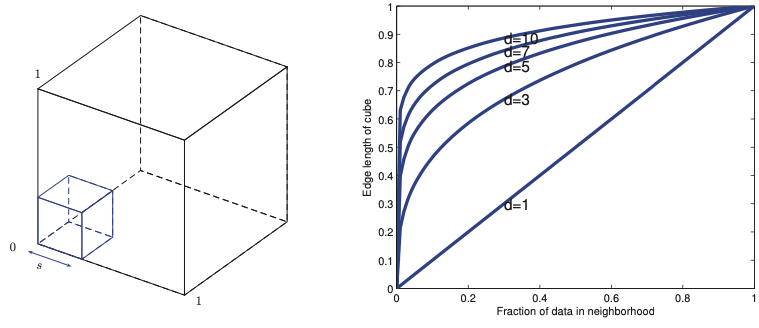
\includegraphics[width=0.8\linewidth]{figures/intro-cube-overfitting.png}}
}
\caption{We embed a small cube within a unit cube (left) and assess a lenght of the edge of a small cube to cover a fraction of uniformly spread data. Graphs borrowed from~\citet{2012-Murphy}.}
\label{fig:cube-in-cube}
\end{figure}


\printbibliography[heading=subbibliography]
\end{refsection}

\end{document}
